\documentclass[twocolumn]{article}
\usepackage[]{float}
\usepackage[]{graphicx}


%opening
\title{}
\author{}

\begin{document}

\maketitle

We need to test the A, B, D functions implemented. We test them by setting only one pair of values to a non-zero value.

\section{Gamov-Teller ($J_i$ = 1; $J_f$ = 2)}

We first analyse the simple case: a Gamov-Teller transition. (For a Fermi transition we get trivial results, since all terms in A, B and D are prop to $M_{GT} = 0$). In this case, we only need to consider the terms prop to $M^2_{GT}$, terms prop to $M_F = 0$ can be ignored and so do terms prop to $\delta_{J_i,J_f}$. 

\subsection{First Test: 0 vs NaN vs cte vs $\neq$ cte}

Since we need do characterise each pair and check if the values given are correct for the whole energy, we'd need to compare the output with a graph. To reduce the amount of graphs, we can inspect first if the functions will return 0, be undefined ($\xi$ in the denominator of the expressions can be 0), return a non-zero constant value or a variable one. 

We check the results of the maximum function from the test, printed in the terminal. If maximum returns -1, it implies all values are NaN (because of 1/0 division) and thus fail the comparison with -1, the starting value of the function. If maximum is 0, all computed values must be zero. The output in terminal is also configured to show if the function is constant across the domain we plotted or not.

\subsubsection{Real Terms}

For a first test, we set to +1 only the two constants we select in the pair, rest are set to 0. Here are the results.

\begin{table}[H]
	\begin{tabular}{|c|c|c|c|c|c|c|c|}
		\hline
		CS & $\xi $& $A_t$ & $B_t$ & $D_t$ & A & B & D \\
		\hline
		CSP & 0 & NaN & NaN & NaN & NaN & NaN & 0\\
		\hline
		CT & 1 & 0 & 0 & 0 & 0 & 0 & 0\\
		\hline
		CTP & 1 & 0 & 0 & 0 & 0 & 0 & 0\\
		\hline
		CV & 0 & NaN & NaN & NaN & NaN & NaN & 0\\
		\hline
		CVP & 0 & NaN & NaN & NaN & NaN & NaN & 0\\
		\hline
		CA & 1 & 0 & 0 & 0 & 0 & 0 & 0\\
		\hline
		CAP & 1 & 0 & 0 & 0 & 0 & 0 & 0\\
		\hline
	\end{tabular}
	\caption{Results of the test with CS as one of the variables. The first column is the second coupling constant, 2nd is $\xi$; 3rd to 5th are the expectqtion from inspecting the function, 6th to 8th the values from the test}
\end{table}

\begin{table}[H]
	\begin{tabular}{|c|c|c|c|c|c|c|c|}
		\hline
		CSP & $\xi $& $A_t$ & $B_t$ & $D_t$ & A & B & D \\
		\hline
		CT & 1 & 0 & 0 & 0 & 0 & 0 & 0\\
		\hline
		CTP & 1 & 0 & 0 & 0 & 0 & 0 & 0\\
		\hline
		CV & 0 & NaN & NaN & NaN & NaN & NaN & 0\\
		\hline
		CVP & 0 & NaN & NaN & NaN & NaN & NaN & 0\\
		\hline
		CA & 1 & 0 & 0 & 0 & 0 & 0 & 0\\
		\hline
		CAP & 1 & 0 & 0 & 0 & 0 & 0 & 0\\
		\hline
	\end{tabular}
\end{table}

\begin{table}[H]
	\begin{tabular}{|c|c|c|c|c|c|c|c|}
		\hline
		CT & $\xi $& $A_t$ & $B_t$ & $D_t$ & A & B & D \\
		\hline
		CTP & 2 & cte & cte & 0 & cte & cte & 0\\
		\hline
		CV & 1 & 0 & 0 & 0 & 0 & 0 & 0\\
		\hline
		CVP & 1 & 0 & 0 & 0 & 0 & 0 & 0\\
		\hline
		CA & 2 & 0 & 0 & 0 & 0 & 0 & 0\\
		\hline
		CAP & 2 & 0 & $\neq$cte & 0 & 0 & $\neq$cte & 0\\
		\hline
	\end{tabular}
\end{table}

\begin{table}[H]
	\begin{tabular}{|c|c|c|c|c|c|c|c|}
		\hline
		CTP & $\xi $& $A_t$ & $B_t$ & $D_t$ & A & B & D \\
		\hline
		CV & 1 & 0 & 0 & 0 & 0 & 0 & 0\\
		\hline
		CVP & 1 & 0 & 0 & 0 & 0 & 0 & 0\\
		\hline
		CA & 2 & 0 & $\neq$cte & 0 & 0 & $\neq$cte & 0\\
		\hline
		CAP & 2 & 0 & 0 & 0 & 0 & 0 & 0\\
		\hline
	\end{tabular}
\end{table}

\begin{table}[H]
	\begin{tabular}{|c|c|c|c|c|c|c|c|}
		\hline
		CV & $\xi $& $A_t$ & $B_t$ & $D_t$ & A & B & D \\
		\hline
		CVP & 0 & NaN & NaN & NaN & NaN & NaN & 0\\
		\hline
		CA & 1 & 0 & 0 & 0 & 0 & 0 & 0\\
		\hline
		CAP & 1 & 0 & 0 & 0 & 0 & 0 & 0\\
		\hline
	\end{tabular}
\end{table}


\begin{table}[H]
	\begin{tabular}{|c|c|c|c|c|c|c|c|}
		\hline
		CVP & $\xi $& $A_t$ & $B_t$ & $D_t$ & A & B & D \\
		\hline
		CA & 1 & 0 & 0 & 0 & 0 & 0 & 0\\
		\hline
		CAP & 1 & 0 & 0 & 0 & 0 & 0 & 0\\
		\hline
	\end{tabular}
\end{table}

\begin{table}[H]
	\begin{tabular}{|c|c|c|c|c|c|c|c|}
		\hline
		CA & $\xi $& $A_t$ & $B_t$ & $D_t$ & A & B & D \\
		\hline
		CAP & 2 & cte & cte & 0 & cte & cte & 0\\
		\hline
	\end{tabular}
\end{table}

We observe the results agree with the predictions. It should be noted that, because $J_i \neq J_f$, D returns 0 directly with the current implementation, bypassing any division by 0 due to $\xi = 0$. 

\subsubsection{Imaginary Terms}

For a second test, we give the pair the values $c_1 = 0.8 + 0.6i$, $c_2 = 0.6 - 0.8i$. These are chosen so that the modulus is 1, giving us integer values for $\xi$. The values are also chosen to prove only the imaginary terms, as $c_1\overline{c_2} = (0.8+0.6i)(0.6+0.8i) = i$, so any term on the real part will be zero. This also implies B = 0 in this test.

\begin{table}[H]
	\begin{tabular}{|c|c|c|c|c|c|c|c|}
		\hline
		CS & $\xi $& $A_t$ & $B_t$ & $D_t$ & A & B & D \\
		\hline
		CSP & 0 & NaN & NaN & NaN & NaN & NaN & 0\\
		\hline
		CT & 1 & 0 & 0 & 0 & 0 & 0 & 0\\
		\hline
		CTP & 1 & 0 & 0 & 0 & 0 & 0 & 0\\
		\hline
		CV & 0 & NaN & NaN & NaN & NaN & NaN & 0\\
		\hline
		CVP & 0 & NaN & NaN & NaN & NaN & NaN & 0\\
		\hline
		CA & 1 & 0 & 0 & 0 & 0 & 0 & 0\\
		\hline
		CAP & 1 & 0 & 0 & 0 & 0 & 0 & 0\\
		\hline
	\end{tabular}
\end{table}

\begin{table}[H]
	\begin{tabular}{|c|c|c|c|c|c|c|c|}
		\hline
		CSP & $\xi $& $A_t$ & $B_t$ & $D_t$ & A & B & D \\
		\hline
		CT & 1 & 0 & 0 & 0 & 0 & 0 & 0\\
		\hline
		CTP & 1 & 0 & 0 & 0 & 0 & 0 & 0\\
		\hline
		CV & 0 & NaN & NaN & NaN & NaN & NaN & 0\\
		\hline
		CVP & 0 & NaN & NaN & NaN & NaN & NaN & 0\\
		\hline
		CA & 1 & 0 & 0 & 0 & 0 & 0 & 0\\
		\hline
		CAP & 1 & 0 & 0 & 0 & 0 & 0 & 0\\
		\hline
	\end{tabular}
\end{table}

\begin{table}[H]
	\begin{tabular}{|c|c|c|c|c|c|c|c|}
		\hline
		CT & $\xi $& $A_t$ & $B_t$ & $D_t$ & A & B & D \\
		\hline
		CTP & 2 & 0 & 0 & 0 & 0 & 0 & 0\\
		\hline
		CV & 1 & 0 & 0 & 0 & 0 & 0 & 0\\
		\hline
		CVP & 1 & 0 & 0 & 0 & 0 & 0 & 0\\
		\hline
		CA & 2 & 0 & 0 & 0 & 0 & 0 & 0\\
		\hline
		CAP & 2 & $\neq$cte & 0 & 0 & $\neq$cte & 0 & 0\\
		\hline
	\end{tabular}
\end{table}

\begin{table}[H]
	\begin{tabular}{|c|c|c|c|c|c|c|c|}
		\hline
		CTP & $\xi $& $A_t$ & $B_t$ & $D_t$ & A & B & D \\
		\hline
		CV & 1 & 0 & 0 & 0 & 0 & 0 & 0\\
		\hline
		CVP & 1 & 0 & 0 & 0 & 0 & 0 & 0\\
		\hline
		CA & 2 & $\neq$cte & 0 & 0 & $\neq$cte & 0 & 0\\
		\hline
		CAP & 2 & 0 & 0 & 0 & 0 & 0 & 0\\
		\hline
	\end{tabular}
\end{table}

\begin{table}[H]
	\begin{tabular}{|c|c|c|c|c|c|c|c|}
		\hline
		CV & $\xi $& $A_t$ & $B_t$ & $D_t$ & A & B & D \\
		\hline
		CVP & 0 & NaN & NaN & NaN & NaN & NaN & 0\\
		\hline
		CA & 1 & 0 & 0 & 0 & 0 & 0 & 0\\
		\hline
		CAP & 1 & 0 & 0 & 0 & 0 & 0 & 0\\
		\hline
	\end{tabular}
\end{table}

\begin{table}[H]
	\begin{tabular}{|c|c|c|c|c|c|c|c|}
		\hline
		CVP & $\xi $& $A_t$ & $B_t$ & $D_t$ & A & B & D \\
		\hline
		CA & 1 & 0 & 0 & 0 & 0 & 0 & 0\\
		\hline
		CAP & 1 & 0 & 0 & 0 & 0 & 0 & 0\\
		\hline
	\end{tabular}
\end{table}

\begin{table}[H]
	\begin{tabular}{|c|c|c|c|c|c|c|c|}
		\hline
		CA & $\xi $& $A_t$ & $B_t$ & $D_t$ & A & B & D \\
		\hline
		CAP & 2 & 0 & 0 & 0 & 0 & 0 & 0\\
		\hline
	\end{tabular}
	\caption{Results of the test with CS as one of the variables. The first column is the second coupling constant, 2nd is $\xi$; 3rd to 5th are the expectqtion from inspecting the function, 6th to 8th the values from the test}
\end{table}

The results obtained match the predictions once more, confirming the function works

\subsection{Second Test: correct numerical values}.

Out of the combinations selected as non-zero constant and variable, we do the computations to check the validity. In our test, we have used $Z=14$ and assumed the transition is $\beta^-$, that is $betaType=+1$, with $Q = 2000\mathrm{keV}$. From the choice of $J_i = 1$ and $J_f = 2$, $$\lambda_{J_i,J_f}=-\frac{J_i}{J_i+1} = -0.5$$. We can note additionaly from the tables $\xi = 2$ in all the cases.

\subsubsection{Constant-Valued Terms}

\subsubsection*{ct=1,ctp=1}

Here both A and B are constant. From the formulae, the only non-zero terms are 
$$A = \frac{2}{\xi}|M_{GT}|^2\lambda_{J_i,J_f}Re(C_T\overline{C_T'}) = -0.5$$
$$B = \frac{2}{\xi}|M_{GT}|^2\lambda_{J_i,J_f}Re(C_T\overline{C_T'}) = -0.5$$
The print in terminal already confirms the absolute value, while looking at the files we see A = B = -0.5, confirming the results

\subsubsection*{ca=1,cap=1}

Here both A and B are constant. From the formulae, the only non-zero terms are 
$$A = \frac{2}{\xi}|M_{GT}|^2\lambda_{J_i,J_f}Re(-C_A\overline{C_A'}) = 0.5$$
$$B = \frac{2}{\xi}|M_{GT}|^2\lambda_{J_i,J_f}Re(C_A\overline{C_A'}) =-0.5$$
We obtain the results we calculated as well.

\subsubsection{Variable Terms}

We plot now the values obtained for non-constant terms and compare them with their analytical expressions.

\subsubsection*{ct=1,cap=1}

The only non-zero term in this product is

$$B= \frac{2}{\xi}|M_{GT}|^2\lambda_{J_i,J_f}\frac{\gamma m_e}{E}Re(C_T\overline{C_A'})$$

with $$\gamma = \sqrt{1-(\alpha Z)^2}$$

The result can be seen in Figure 1. The points land on the curve precisely for all three parameters A,B and D

\begin{figure}
	\centering
	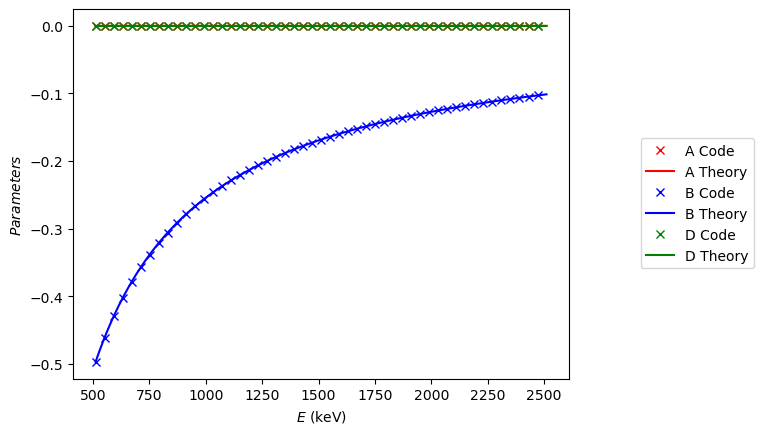
\includegraphics[width=\columnwidth]{plots/ctcap_real_gt_result.png}
	\caption{Coeficients A, B, D with respect to energy of the electron for a Gamov-Teller Z = 14 Q = 2000 keV decay with non-zero coupling constants ct=1,cap=1}
\end{figure}

\subsubsection*{ctp=1,ca=1}

The relevant term is in this case

$$B= \frac{2}{\xi}|M_{GT}|^2\lambda_{J_i,J_f}\frac{\gamma m_e}{E}Re(C_T'\overline{C_A})$$

with the gamma as defined previously. The expression is equivalent to the case ct=1,cap=1 seen previously and as such the resulting plot (Figure 2) is identical.

\begin{figure}
	\centering
	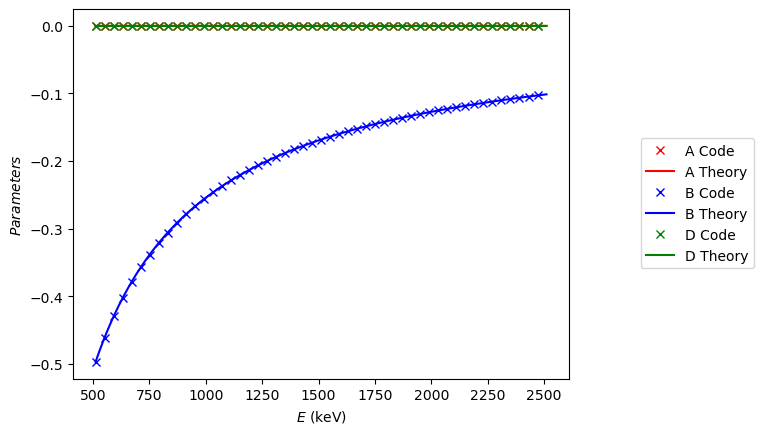
\includegraphics[width=\columnwidth]{plots/ctcap_real_gt_result.png}
	\caption{Coeficients A, B, D with respect to energy of the electron for a Gamov-Teller Z = 14 Q = 2000 keV decay  with non-zero coupling constants ctp=1,ca=1.}
\end{figure}

\subsubsection*{ct=0.8+0.6i,cap=0.6-0.8i}

The relevant term in this case is 

$$A= \frac{2}{\xi}|M_{GT}|^2\lambda_{J_i,J_f}\frac{\alpha Z}{v_e}\cdot Im(C_T\overline{C_A'})$$

with $$v_e = \frac{p_e}{E} = \sqrt{1-\frac{m^2_e}{E^2}}$$

\begin{figure}
	\centering
	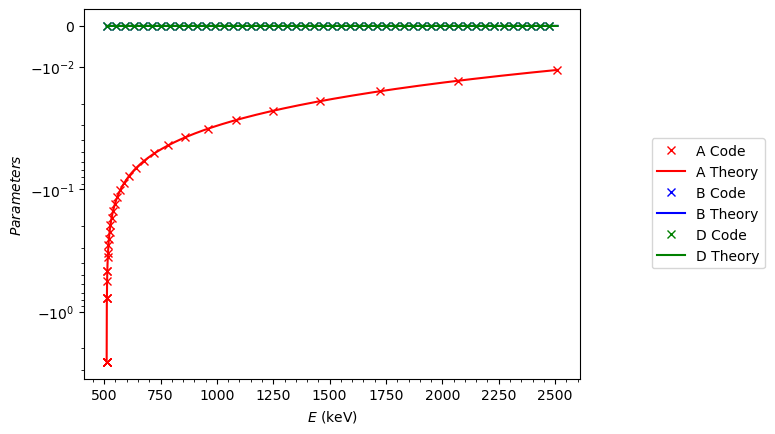
\includegraphics[width=\columnwidth]{plots/ctcap_comp_gt_result.png}
	\caption{Coeficients A, B, D with respect to energy of the electron for a Gamov-Teller Z = 14 Q = 2000 keV decay with non-zero coupling constants ct=0.8+0.6i,cap=0.6-0.8i}
\end{figure}

\subsubsection*{ctp=0.8+0.6i,ca=0.6-0.8i}

The relevant term in this case is 

$$A= \frac{2}{\xi}|M_{GT}|^2\lambda_{J_i,J_f}\frac{\alpha Z}{v_e}\cdot Im(C_T'\overline{C_A})$$

with the gamma as defined previously. The expression is equivalent to the case ct=0.8+0.6i,cap=0.6-0.8i seen previously and as such the resulting plot (Figure 4) is identical.


\begin{figure}
	\centering
	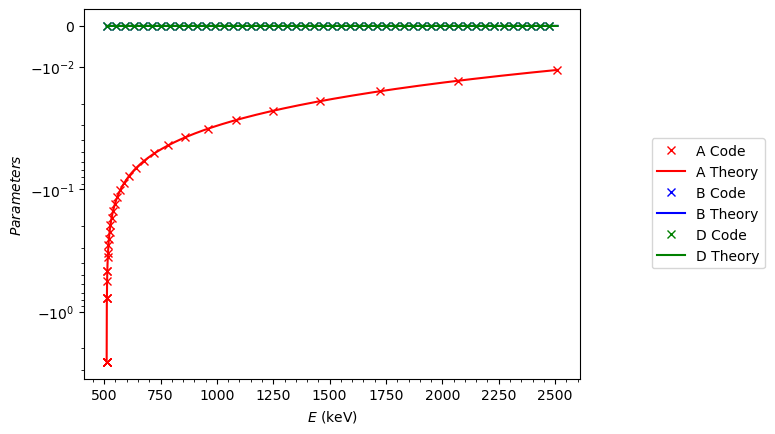
\includegraphics[width=\columnwidth]{plots/ctcap_comp_gt_result.png}
	\caption{Coeficients A, B, D with respect to energy of the electron for a Gamov-Teller Z = 14 Q = 2000 keV decay  with non-zero coupling constants ctp=0.8+0.6i,ca=0.6-0.8i.}
\end{figure}

\section{Mixed Decay ($J_i$ = $J_f$ = 1)}

We now consider a mixed transition, where both Gamov-Teller and Fermi terms are present. In this case, we need to consider both the terms prop to $M^2_{GT}$, and the terms prop to $M_F$ and $\delta_{J_i,J_f}$. 


\subsection{First Test: 0 vs NaN vs cte vs $\neq$ cte}

We perform the same checks initially as in the pure Gamov-Teller case. We once more check the results of the maximum function (=0, =NaN (shown in the results as -1) or $\neq$0) and the characterisation of the function (constant or variable) from the test. 

\subsubsection{Real Values}

For a first test, we set to +1 only the two constants we select in the pair, rest are set to 0. Because of the choice of constants, $\xi=2$. As a consequence, no NaN values can be obtained . Here are the results.

\begin{table}[H]
	\begin{tabular}{|c|c|c|c|c|c|c|}
		\hline
		CS & $A_t$ & $B_t$ & $D_t$ & A & B & D \\
		\hline
		CSP & 0 & 0 & 0 & 0 & 0 & \\
		\hline
		CT & 0 & 0 & 0 & 0 & 0 & 0\\
		\hline
		CTP & cte & cte & 0 & cte& cte & 0\\
		\hline
		CV & 0 & 0 & 0 & 0 & 0 & 0 \\
		\hline
		CVP & 0 & 0 & 0 & 0 & 0 & 0\\
		\hline
		CA & 0 & 0 & $\neq$cte & 0 & 0 & $\neq$cte\\
		\hline
		CAP & 0 & $\neq$cte & 0 & 0 & $\neq$cte & 0\\
		\hline
	\end{tabular}
	\caption{Results of the test with CS as one of the variables. The first column is the second coupling constant, 2nd is $\xi$; 3rd to 5th are the expectation from inspecting the function, 6th to 8th the values from the test}
\end{table}

\begin{table}[H]
	\begin{tabular}{|c|c|c|c|c|c|c|}
		\hline
		CSP & $A_t$ & $B_t$ & $D_t$ & A & B & D \\
		\hline
		CT & cte & cte & 0 & cte & cte  &0 \\
		\hline
		CTP & 0 & 0 & 0 & 0 & 0 & 0\\
		\hline
		CV & 0 & 0 & 0 & 0 & 0 & 0\\
		\hline
		CVP & 0 & 0 & 0 & 0 & 0 & 0\\
		\hline
		CA & 0 & $\neq$cte & 0 & 0 & $\neq$cte & 0\\
		\hline
		CAP & 0 & 0 & $\neq$cte & 0 & 0 & $\neq$cte \\
		\hline
	\end{tabular}
\end{table}

\begin{table}[H]
	\begin{tabular}{|c|c|c|c|c|c|c|}
		\hline
		CT & $A_t$ & $B_t$ & $D_t$ & A & B & D \\
		\hline
		CTP & cte & cte & 0 & cte & cte & 0\\
		\hline
		CV & 0 & 0 & $\neq$cte & 0 & 0 & $\neq$cte\\
		\hline
		CVP & 0 & $\neq$cte & 0 & 0 & $\neq$cte & 0\\
		\hline
		CA & 0 & 0 & 0 & 0 & 0 & 0\\
		\hline
		CAP & 0 & $\neq$cte & 0 & 0 & $\neq$cte & 0\\
		\hline
	\end{tabular}
\end{table}

\begin{table}[H]
	\begin{tabular}{|c|c|c|c|c|c|c|}
		\hline
		CTP & $A_t$ & $B_t$ & $D_t$ & A & B & D \\
		\hline
		CV & 0 & $\neq$cte & 0 & 0 & $\neq$cte & 0 \\
		\hline
		CVP & 0 & 0 & $\neq$cte & 0 & 0 & $\neq$cte\\
		\hline
		CA & 0 & $\neq$cte & 0 & 0 & $\neq$cte & 0 \\
		\hline
		CAP & 0 & 0 & 0 & 0 & 0 & 0\\
		\hline
	\end{tabular}
\end{table}

\begin{table}[H]
	\begin{tabular}{|c|c|c|c|c|c|c|}
		\hline
		CV & $A_t$ & $B_t$ & $D_t$ & A & B & D \\
		\hline
		CVP & 0 & 0 & 0 & 0 & 0 & 0\\
		\hline
		CA & 0 & 0 & 0 & 0 & 0 & 0\\
		\hline
		CAP & cte & cte & 0 & cte & cte & 0\\
		\hline
	\end{tabular}
\end{table}


\begin{table}[H]
	\begin{tabular}{|c|c|c|c|c|c|c|}
		\hline
		CVP & $A_t$ & $B_t$ & $D_t$ & A & B & D \\
		\hline
		CA & cte & cte & 0 & cte & cte & 0\\
		\hline
		CAP & 0 & 0 & 0 & 0 & 0 & 0\\
		\hline
	\end{tabular}
\end{table}

\begin{table}[H]
	\begin{tabular}{|c|c|c|c|c|c|c|}
		\hline
		CA & $A_t$ & $B_t$ & $D_t$ & A & B & D \\
		\hline
		CAP & cte & cte & 0 & cte & cte & 0\\
		\hline
	\end{tabular}
\end{table}

All results agreed already from the first implementation

\subsubsection{Complex Values}

For a second test, we give the pair the values $c_1 = 0.8 + 0.6i$, $c_2 = 0.6 - 0.8i$. These are chosen so that the modulus is 1, giving us integer values for $\xi$. The values are also chosen to prove only the imaginary terms, as $c_1\overline{c_2} = (0.8+0.6i)(0.6+0.8i) = i$, so any term on the real part will be zero. This also implies B = 0 in this test.

\begin{table}[H]
	\begin{tabular}{|c|c|c|c|c|c|c|}
		\hline
		CS & $A_t$ & $B_t$ & $D_t$ & A & B & D \\
		\hline
		CSP & 0 & 0 & 0 & 0 & 0 & 0\\
		\hline
		CT & 0 & 0 & cte & 0 & 0 & cte\\
		\hline
		CTP & 0 & 0 & 0 & 0 & 0 & 0\\
		\hline
		CV & 0 & 0 & 0 & 0 & 0 & 0\\
		\hline
		CVP & 0 & 0 & 0 & 0 & 0 & 0\\
		\hline
		CA & 0 & 0 & 0 & 0 & 0 & 0\\
		\hline
		CAP & $\neq$cte & 0 & 0 & $\neq$cte$^\ast$ & 0 & 0\\ %review the paper -> result: paper ok, implementation missing a term
		\hline
	\end{tabular}
	\caption{Results of the test with CS as one of the variables. The first column is the second coupling constant, 2rd to 4th are the expected results from inspecting the function, 5th to 7th the values from the test}
\end{table}

\begin{table}[H]
	\begin{tabular}{|c|c|c|c|c|c|c|}
		\hline
		CSP & $A_t$ & $B_t$ & $D_t$ & A & B & D \\
		\hline
		CT & 0 & 0 & 0 & 0 & 0  & 0\\
		\hline
		CTP& 0 & 0 & cte & 0 & 0 & cte\\
		\hline
		CV & 0 & 0 & 0 & 0 & 0 & 0\\
		\hline
		CVP & 0 & 0 & 0 & 0 & 0 & 0\\
		\hline
		CA & $\neq$cte & 0 & 0 & $\neq$cte$^\ast$ & 0 & 0\\  %review the paper
		\hline
		CAP & 0 & 0 & 0 & 0 & 0 & 0\\
		\hline
	\end{tabular}
\end{table}

\begin{table}[H]
	\begin{tabular}{|c|c|c|c|c|c|c|}
		\hline
		CT & $A_t$ & $B_t$ & $D_t$ & A & B & D \\
		\hline
		CTP & 0 & 0 & 0 & 0 & 0 & 0\\
		\hline
		CV & 0 & 0 & 0 & 0 & 0 & 0\\
		\hline
		CVP & $\neq$cte & 0 & 0 & $\neq$cte$^\ast$ & 0 & 0\\ %review the paper
		\hline
		CA & 0 & 0 & 0 & 0 & 0 & 0\\
		\hline
		CAP & $\neq$cte & 0 & 0 & $\neq$cte & 0 & 0\\
		\hline
	\end{tabular}
\end{table}

\begin{table}[H]
	\begin{tabular}{|c|c|c|c|c|c|c|}
		\hline
		CTP & $A_t$ & $B_t$ & $D_t$ & A & B & D \\
		\hline
		CV & $\neq$cte & 0 & 0 & $\neq$cte$^\ast$ & 0 & 0\\
		\hline %review
		CVP & 0 & 0 & 0 & 0 & 0 & 0\\
		\hline
		CA & $\neq$cte & 0 & 0 & $\neq$cte & 0 & 0\\
		\hline
		CAP & 0 & 0 & 0 & 0 & 0 & 0\\
		\hline
	\end{tabular}
\end{table}

\begin{table}[H]
	\begin{tabular}{|c|c|c|c|c|c|c|}
		\hline
		CV & $A_t$ & $B_t$ & $D_t$ & A & B & D \\
		\hline
		CVP & 0 & 0 & 0 & 0 & 0 & 0\\
		\hline
		CA & 0 & 0 & cte & 0 & 0 & cte\\
		\hline
		CAP & 0 & 0 & 0 & 0 & 0 & 0\\
		\hline
	\end{tabular}
\end{table}


\begin{table}[H]
	\begin{tabular}{|c|c|c|c|c|c|c|}
		\hline
		CVP & $A_t$ & $B_t$ & $D_t$ & A & B & D \\
		\hline
		CA & 0 & 0 & 0 & 0 & 0 & 0 \\
		\hline
		CAP & 0 & 0 & cte & 0 & 0 & cte\\
		\hline
	\end{tabular}
\end{table}

\begin{table}[H]
	\begin{tabular}{|c|c|c|c|c|c|c|}
		\hline
		CA & $A_t$ & $B_t$ & $D_t$ & A & B & D \\
		\hline
		CAP & 0 & 0 & 0 & 0 & 0 & 0\\
		\hline
	\end{tabular}
\end{table}

The results at first test didn't match for the values marked in $^\ast$ because of a missing term in the imaginary part of the $\delta_{J_i,J_f}$ term. The error was not found until this test because it wouldn't yield anything in all previous tests. 

\subsection{Second Test: correct numerical values}.

As in the case of the Gamov-Teller transition, we procede to analyse more closely the numerical results. We use the same parameters for the reaction, noting the change in the value of $\lambda_{J_i,J_f}$  

$$\lambda_{J_i,J_f} = \frac{1}{J_i+1} = 0.5$$

From this, we should expect a change in sign but same absolute value for the pairs of coupling constants we checked the numerical values of in detail. This can be seen as there is no extra term in A, B or D proportional to their product

\subsubsection{Constant-Valued Terms}

First the pairs we saw in the Gamov-Teller decay

\subsubsection*{ct=1,ctp=1}

Here both A and B are constant. From the formulae, the only non-zero terms are 
$$A = \frac{2}{\xi}|M_{GT}|^2\lambda_{J_i,J_f}Re(C_T\overline{C_T'}) = 0.5$$
$$B = \frac{2}{\xi}|M_{GT}|^2\lambda_{J_i,J_f}Re(C_T\overline{C_T'}) = 0.5$$
The print in terminal already confirms the absolute value, while looking at the files we see A = B = 0.5. As noted, this value has opposite sign to the Gamov-Teller case because we have no new non-zero terms proportional to $(C_T\overline{C_T'})$

\subsubsection*{ca=1,cap=1}

Both A and B are constant as well. From the formulae, the only non-zero terms are 
$$A = \frac{2}{\xi}|M_{GT}|^2\lambda_{J_i,J_f}Re(-C_A\overline{C_A'}) = -0.5$$
$$B = \frac{2}{\xi}|M_{GT}|^2\lambda_{J_i,J_f}Re(C_A\overline{C_A'}) = 0.5$$
From the code we reproduce this results as well.

\subsubsection*{cs=1,ctp=1\\csp=1,ct=1\\cv=1,cap=1\\cv=1,cap=1}

Both A and B are constant for all these pairs. From the formulae, the only non-zero terms are 
$$A = \frac{2}{\xi}M_FM_{GT}\delta_{J_i,J_f}\sqrt{\frac{J_i}{J_i+1}}$$$$ Re(C_S\overline{C_T'}+C_S'\overline{C_T}-C_V\overline{C_A'}-C_V'\overline{C_A})$$
$$B = \frac{2}{\xi}M_FM_{GT}\delta_{J_i,J_f}\sqrt{\frac{J_i}{J_i+1}}$$$$ Re(-C_S\overline{C_T'}-C_S'\overline{C_T}-C_V\overline{C_A'}-C_V'\overline{C_A})$$

For all pairs, substituting each pair of coefficients results in a value that has the same absolute value, $1/\sqrt{2} \approx 0.707107$. This value is also the maximum, so it can be confirmed in the terminal output (up to 6 decimal places). Inspecting the files we see a positive sign for A with the (cs,ctp) and (csp,ct) pairs, and negative for A with the (cv,cap) and (cvp,ca) pairs and all values of B. This agrees with the results

\subsubsection*{cs=0.8+0.6i,ct=0.6-0.8i;\\csp=0.8+0.6i,ctp=0.6-0.8i;\\cv=0.8+0.6i,ca=0.6-0.8i;\\cvp=0.8+0.6i,cap=0.6-0.8i}

The only non-zero coefficient for all this pairs is D. The relevant term is

$$D = \frac{2}{\xi}M_FM_{GT}\delta_{J_i,J_f}\sqrt{\frac{J_i}{J_i+1}}\cdot$$$$ \cdot Im(C_S\overline{C_T}+C_S'\overline{C_T'}-C_V\overline{C_A}-C_V'\overline{C_A'})$$

For all pairs, the result has the same absolue value, $1/\sqrt{2} \approx 0.70711$. This result can be seen printed on terminal while we execute the test. The sign of the result can be inspected in the output files, being positive for the (cs,ct) and (csp,ctp) pairs and negative for the other 2, (cv,ca) and (cvp,cap). Here we realise there is a flipped sign in the definition, which we correct.


\subsubsection{Variable Terms}

 \subsubsection*{ct=1,cap=1;\\ctp=1,ca=1}
 
 The relevant term is in this case, for both pairs, is
 
 $$B= \frac{2}{\xi}|M_{GT}|^2\lambda_{J_i,J_f}\frac{\gamma m_e}{E}Re(C_T\overline{C_A'}+C_T'\overline{C_A})$$
 
 with $$\gamma = \sqrt{1-(\alpha Z)^2}$$
 
 For both figures we obtain the same plot, figure 5.
 
 \begin{figure}
 	\centering
 	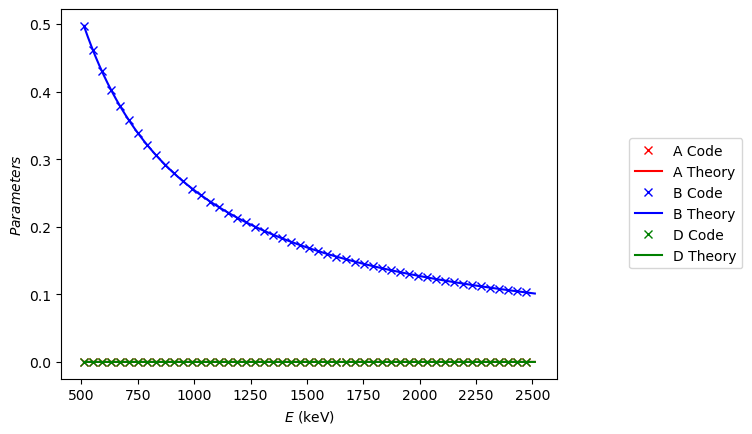
\includegraphics[width=\columnwidth]{plots/ctcap_real_mixed_result.png}
 	\caption{Coeficients A, B, D with respect to energy of the electron for a mixed Z = 14 Q = 2000 keV decay  with non-zero coupling constants ctp=1,ca=1.}
 \end{figure}
 
 \subsubsection*{ct=0.8+0.6i,cap=0.6-0.8i;\\ctp=0.8+0.6i,ca=0.6-0.8i}
 
 The relevant term in this case is 
 
 $$A= \frac{2}{\xi}|M_{GT}|^2\lambda_{J_i,J_f}\frac{\alpha Z}{v_e}\cdot Im(C_T\overline{C_A'}+C_T'\overline{C_A})$$
 
 For both pairs we obtain the same plot, figure 6.
 
 \begin{figure}
 	\centering
 	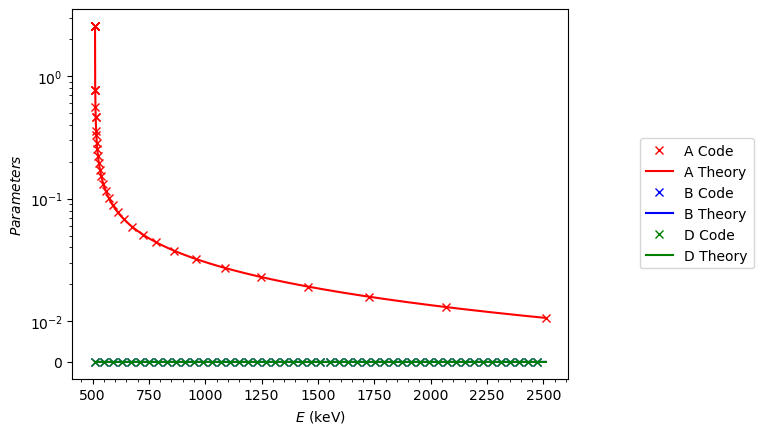
\includegraphics[width=\columnwidth]{plots/ctcap_comp_mixed_result.png}
 	\caption{Coeficients A, B, D with respect to energy of the electron for a mixed Z = 14 Q = 2000 keV decay with non-zero coupling constants ct=0.8+0.6i,cap=0.6-0.8i}
 \end{figure}
 
 \subsubsection*{cs=1,cap=1;\\csp=1,ca=1;\\ct=1,cvp=1;\\ctp=1,cv=1}

 The relevant term in this case is 

 $$B = \frac{2}{\xi}M_FM_{GT}\delta_{J_i,J_f}\sqrt{\frac{J_i}{J_i+1}}\frac{\gamma m_e}{E}$$$$Re(C_S\overline{C_A'}+C_S'\overline{C_A}+C_T\overline{C_V'}+C_T'\overline{C_V})$$

 For all for pairs we obtain the same plot, figure 7. The initial result disagreed by a factor of two, coming from a missing 2 in the formula, which has now been corrected.
 
  \begin{figure}
 	\centering
 	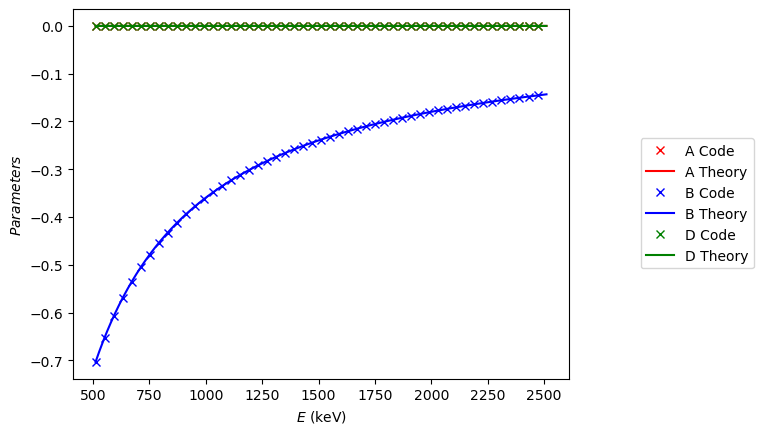
\includegraphics[width=\columnwidth]{plots/cscap_real_mixed_result.png}
 	\caption{Coeficients A, B, D with respect to energy of the electron for a mixed Z = 14 Q = 2000 keV decay with non-zero coupling constants cs=1,cap=1}
 \end{figure}
 
 
\subsubsection*{cs=1,ca=1;\\csp=1,cap=1;\\ct=1,cv=1;\\ctp=1,cvp=1}

The relevant term in this case is 

$$D = \frac{2}{\xi}M_FM_{GT}\delta_{J_i,J_f}\sqrt{\frac{J_i}{J_i+1}}\frac{\alpha Z }{v_e}$$$$Re(C_S\overline{C_A}+C_S'\overline{C_A'}C_T\overline{C_V'}+C_T'\overline{C_V})$$

For all for pairs we obtain the same plot, figure 8. The plotted points agree with the curve, without any necessary changes to the code.

\begin{figure}
	\centering
	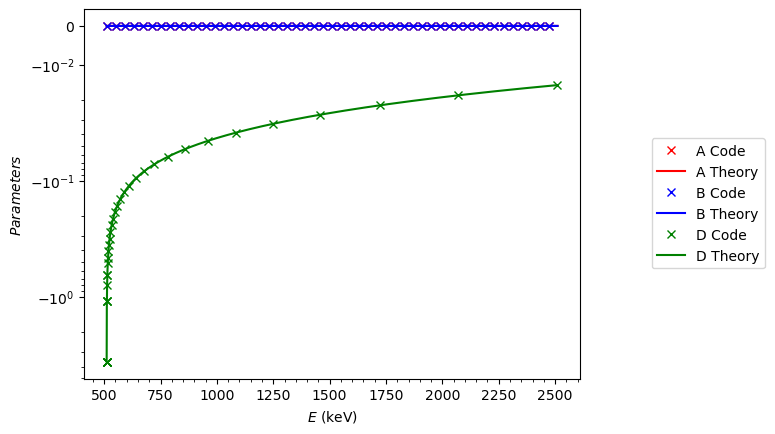
\includegraphics[width=\columnwidth]{plots/csca_real_mixed_result.png}
	\caption{Coeficients A, B, D with respect to energy of the electron for a mixed Z = 14 Q = 2000 keV decay with non-zero coupling constants cs=1,cap=1}
\end{figure}

\subsubsection*{cs=0.8+0.6i,cap=0.6-0.8i;\\csp=0.8+0.6i,ca=0.6-0.8i;\\ct=0.8+0.6i,cvp=0.6-0.8i;\\ctp=0.8+0.6i,cv=0.6-0.8i}

The only function that is non-zero is A, specifically the term proportional to the imaginary part of the product of coupling constants and proportional as well to $M_F$


 $$A = \frac{2}{\xi}M_FM_{GT}\delta_{J_i,J_f}\sqrt{\frac{J_i}{J_i+1}}\frac{\alpha Z }{v_e}$$$$Im(C_S\overline{C_A'}+C_S'\overline{C_A}+C_T\overline{C_V'}+C_T'\overline{C_V})$$

For all for pairs we obtain the same plot, figure 9. The plotted points agree with the curve, without any necessary changes to the code.

\begin{figure}
	\centering
	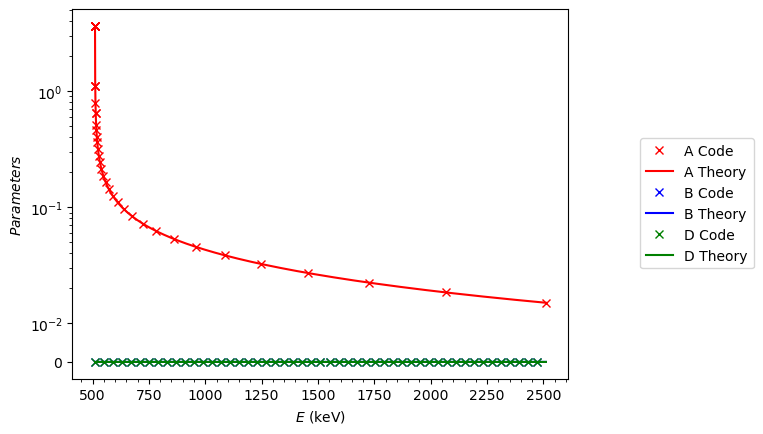
\includegraphics[width=\columnwidth]{plots/cscap_comp_mixed_result.png}
	\caption{Coeficients A, B, D with respect to energy of the electron for a mixed Z = 14 Q = 2000 keV decay with non-zero coupling constants cs=1,cap=1}
\end{figure}

\end{document}





